\documentclass{article}
\usepackage[utf8]{inputenc}
\usepackage[spanish]{babel}
\usepackage{graphicx}
\usepackage{booktabs}
\usepackage{amsmath, amssymb}
\usepackage{geometry}
\usepackage{hyperref}
\usepackage{caption}
\usepackage{enumitem}
\usepackage{multirow}
\usepackage{float}
\usepackage{fancyhdr} % Paquete para encabezados personalizados
\usepackage{parskip}
\usepackage{tcolorbox}
\usepackage{bold-extra}
\usepackage{array} % Para definir ancho de columnas y word wrapping
\usepackage{makecell} % Para ajustar texto dentro de las celdas
\usepackage{ulem}



\setlength{\parskip}{1em}  % Ajusta la distancia entre párrafos
\setlist[itemize]{noitemsep}
%\setlist[enumerate]{noitemsep}
\captionsetup[figure]{labelfont=bf}
\captionsetup[table]{labelfont=bf}
\geometry{margin=1.3in, headheight=30pt}
\addtolength{\topmargin}{-6.23604pt}

\title{Desarrollo de un sistema de programación automatizada de tareas de mantenimiento en la industria minera}
\date{}

\pagestyle{fancy} 
\fancyhf{} 
\lhead{
\includegraphics[width=6cm]{imgs/UC Logo.png}\vspace{1.5mm}} 
\rhead{Emilio Bravo Maturana\\
Magíster en Inteligencia Artificial (c)\vspace{3.5mm}}
\renewcommand{\headrulewidth}{0.4pt} 
\cfoot{\thepage} % Número de página centrado en el pie de página
\renewcommand{\footrulewidth}{0.4pt} % Línea en el pie de página (opcional)

\begin{document}

\begin{titlepage}
\newcommand{\HRule}{\rule{\linewidth}{0.5mm}}
\center
\textsc{\LARGE Pontificia Universidad Católica de Chile}\\[1cm] 
\textsc{\large Magister en Inteligencia Artificial}\\[0.5cm] 
\HRule \\[0.4cm]
\huge \textsc{Desarrollo de un sistema de programación automatizada de tareas de mantenimiento en la industria minera}\\[0.1cm]
\HRule \\[1cm]
\large\textsc{Emilio Bravo Maturana\\\emph{Profesor Guía: }Rodrigo Sandoval Urrich}\\[1cm]

\includegraphics[scale=0.2]{imgs/UC Logo Grande.png}\\[1cm]
\vfill
{\large\emph{Santiago, Chile. \\ Diciembre 2024 }}\\[2cm]


\end{titlepage}

{\bfseries\scshape Título}\\[.25cm]
Desarrollo de un sistema de programación automatizada de tareas de mantenimiento en la industria minera.\\


{\bfseries\scshape Autor}\\[.25cm]
Emilio Bravo Maturana\\

{\bfseries\scshape Temática}\\[.25cm]
Programación de Tareas, Algoritmos de Optimización, Resource-Constrained Project Scheduling Problem (RCPSP), Constraint Programming.

\newpage

\section*{Resumen}
El mantenimiento eficiente de equipos es crucial para garantizar la continuidad operativa en cualquier industria. Sin embargo, la programación manual de estas actividades es compleja, intensiva en tiempo y propensa a errores debido a las múltiples restricciones y variables involucradas. Esto genera una alta dependencia de personal especializado para llevar a cabo la programación de tareas.

Este proyecto tiene como objetivo principal automatizar el proceso de programación de tareas de mantenimiento, liberando al equipo de programación de trabajo manual intensivo y reduciendo significativamente la ocurrencia de errores. Para ello, el problema se modela como un \textbf{Problema de Programación de Proyectos con Restricciones de Recursos} (RCPSP, por sus siglas en inglés). Una generalización correcta del proceso permite utilizar herramientas de optimización para generar cronogramas que cumplan con todas las restricciones del problema, minimizando la función objetivo y mejorando la eficiencia general.

El enfoque busca diseñar un algoritmo que no solo encuentre soluciones óptimas, sino que también ofrezca rapidez y flexibilidad para adaptarse a cambios intempestivos. A través de un estudio detallado y pruebas exhaustivas, se evaluará el desempeño del modelo en términos de ahorro de tiempo, reducción del uso de recursos computacionales y calidad de las soluciones generadas, con el fin de garantizar una planificación eficiente y confiable.

Este texto enfatiza la automatización, la reducción de errores y la liberación del trabajo manual como objetivos centrales.

\newpage

\tableofcontents
\newpage
%\maketitle 
%\vspace{-10mm}
%\thispagestyle{fancy} 

\section{Introducción}
\subsection{Contexto}
El mantenimiento de equipos es una actividad fundamental en cualquier industria que busca garantizar la continuidad operativa y la eficiencia en sus procesos productivos. Una planificación y programación adecuada de las actividades de mantenimiento no solo previene fallos inesperados, sino que también optimiza el uso de recursos y minimiza costos asociados a tiempos de inactividad. Sin embargo, la programación eficiente de estas actividades representa un desafío significativo debido a las múltiples restricciones y variables involucradas, como la disponibilidad de personal, recursos materiales, prioridades de tareas y la necesidad de evitar sobreasignaciones y tiempos muertos.

Tradicionalmente, la planificación del mantenimiento ha dependido de equipos humanos que, a pesar de su experiencia y conocimiento, enfrentan limitaciones en términos de tiempo y capacidad para manejar grandes volúmenes de datos y restricciones complejas. Este proceso manual es propenso a errores y puede no garantizar una solución óptima que maximice la eficiencia operativa. En este contexto, surge la necesidad de automatizar este proceso mediante el uso de algoritmos de optimización que puedan abordar de manera efectiva la complejidad inherente de la programación de mantenimiento.

El problema de programación de mantenimiento puede modelarse como un Problema de Programación de Proyectos con Restricciones de Recursos (RCPSP), un enfoque clásico en la investigación operativa para resolver problemas de planificación bajo condiciones de recursos limitados. En este modelo, las tareas de mantenimiento se consideran actividades con duraciones definidas, precedencias entre ellas y recursos compartidos, como personal o maquinaria, cuya disponibilidad es limitada. Las restricciones de precedencia aseguran que ciertas tareas no pueden comenzar hasta que otras hayan finalizado, mientras que las restricciones de recursos garantizan que las capacidades disponibles no sean excedidas en ningún momento. 

El objetivo es encontrar una programación que minimice el tiempo total de ejecución (makespan) o que optimice el uso de recursos, lo que resulta en una planificación más eficiente y acorde con las demandas operativas. Modelar el problema de esta forma permite aplicar algoritmos de optimización avanzados, como algoritmos de Constraint Programming, para generar soluciones factibles y eficientes.

El presente proyecto tiene como objetivo principal proponer un algoritmo para automatizar la programación de actividades de mantenimiento, reduciendo tanto el tiempo dedicado al proceso como la ocurrencia de errores. Se evaluarán distintas funciones objetivo para determinar cuál entrega los mejores resultados en términos de eficiencia y calidad de las soluciones generadas. Para ello, se contará con el apoyo del área de mantenimiento de una empresa del rubro minero, quienes proporcionarán datos para realizar las pruebas y ofrecerán retroalimentación durante el desarrollo de la solución. Esta colaboración permitirá ajustar el modelo a las necesidades específicas y desafíos particulares del entorno operativo, asegurando que los resultados sean relevantes y aplicables.


\subsection{Consideraciones}
En el contexto de la empresa de del rubro minero, es importante contextualizar la terminología específica utilizada en la programación de tareas. A continuación, se definen algunos términos relevantes para facilitar la comprensión del problema.

\textbf{Cronograma}: El cronograma es la representación temporal de la programación de todas las actividades a lo largo del tiempo. En este proyecto, el cronograma se materializa en una carta GANTT que muestra todas las tareas con su fecha de inicio, hora de inicio y duración. Es una herramienta clave para visualizar y gestionar la ejecución del mantenimiento.

\textbf{Orden de Trabajo}: Una orden de trabajo es un conjunto de tareas que se deben realizar para cumplir con un objetivo específico, como el mantenimiento de un equipo o vehículo. Estas órdenes de trabajo se ingresan en el sistema ERP de la empresa y sirven para coordinar y gestionar las actividades de mantenimiento o producción.

\textbf{Tareas}: Actividades individuales dentro de una orden de trabajo. Estas tareas pueden tener requisitos de precedencia, es decir, algunas deben completarse antes de que otras puedan comenzar. Cada tarea cuenta con una fecha de inicio más temprana (earliest date), una fecha requerida de finalización, una duración, una cantidad de trabajadores necesaria y recursos específicos que se requieren para su ejecución.

\textbf{Criticidad}: La criticidad clasifica las tareas según su nivel de prioridad, en una escala del 1 al 3. Las tareas con criticidad 1 son las más urgentes y deben programarse primero, ya que es grave si no se completan dentro de su ventana de tiempo. Las tareas con criticidad 2 y 3 son menos prioritarias y pueden permitirse más flexibilidad en su programación.

\textbf{Recursos}: Los recursos son los elementos limitados que se necesitan para ejecutar las tareas. En este problema, se identifican dos tipos principales de recursos: \textit{Cuadrillas} y \textit{Equipos compartidos}.

\textbf{Cuadrilla}: La cuadrilla representa un grupo de trabajo asignado a una tarea específica dentro de la orden de trabajo. Cada cuadrilla tiene un número determinado de trabajadores y sigue un esquema de turnos específico, trabajando un número fijo de horas por día y un determinado número de días a la semana. La cuadrilla es responsable de ejecutar las operaciones asignadas dentro de su turno.

\textbf{Equipos compartidos}: En este proyecto, los equipos compartidos se refieren a los recursos que son utilizados por varias cuadrillas y que tienen una disponibilidad limitada. Estos equipos forman parte de los \textit{Production Resource Tools} (PRT) y son críticos en la programación, ya que su uso debe gestionarse cuidadosamente para evitar conflictos y sobreasignaciones. Ejemplos típicos de estos equipos incluyen grúas, camiones pluma, \textit{boom trucks}, \textit{forklifts}, y alza hombres.

\textbf{Turno}: El turno define el esquema de trabajo de una cuadrilla. Por ejemplo, un turno 7x7 implica 7 días de trabajo seguidos por 7 días de descanso. Otros esquemas, como el 5x2A, 5x2B o 5x2C, representan 5 días de trabajo con 2 días de descanso, donde las letras A, B y C indican diferentes franjas horarias: A cubre las primeras 8 horas del día, B las siguientes 8, y C las últimas. Estos turnos permiten que las cuadrillas cubran las 24 horas del día de manera continua.

\textbf{Planificación}: La planificación es el proceso llevado a cabo por el equipo de planificadores, quienes establecen una ventana de tiempo en la que deben realizarse las tareas de mantenimiento. Este proceso se realiza considerando los requerimientos de las máquinas, los tiempos de los procesos industriales y otros factores relacionados con las operaciones del negocio. Es una etapa inicial que no contempla las restricciones de recursos, sino que establece un marco general para la ejecución de las actividades.

\textbf{Programación}: La programación es el proceso mediante el cual el equipo de programación toma la planificación inicial y organiza las tareas de manera detallada, asignando recursos específicos y fechas exactas. Durante esta etapa, se balancean los recursos disponibles para evitar sobreasignaciones y garantizar que todas las tareas puedan completarse dentro de sus ventanas de tiempo. La programación precisa y eficiente es clave para minimizar errores y optimizar el uso de los recursos.

\section{Descripción detallada y levantamiento del problema}
Con el objetivo de automatizar el proceso de programación de tareas en el rubro minero, se llevó a cabo un estudio de los documentos que norman el proceso de programación de tareas en la empresa colaboradora. Este análisis permitió comprender en detalle cómo funciona la programación de tareas en el contexto operativo, y por qué resulta esencial generalizar dicho proceso en un modelo matemático o computacional. El propósito final es implementar una solución automatizada que utilice un algoritmo de optimización capaz de entregar resultados satisfactorios.

A continuación se presenta una descripción del proceso de programación de tareas en el área de mantenimiento de esta empresa del rubro minero, con el fin de identificar los elementos clave y las restricciones involucradas en el problema.


\subsection{Proceso de Planificación}

Previo al proceso de programación, el equipo de planificación es responsable de definir, con base en los requerimientos de las máquinas, los tiempos de los procesos industriales, y otros factores relacionados con el negocio minero, las ventanas temporales en las que deben ejecutarse las tareas de mantenimiento. Esto da como resultado una planificación inicial sobre la cual se basa el proceso de programación.

La planificación considera los objetivos estratégicos de la mina y prioriza el cumplimiento de los requerimientos operativos. Como resultado, se genera una planificación inicial que indica, para cada tarea, la ventana dentro de la cual debe ser realizada. Sin embargo, este proceso no contempla las restricciones de recursos (personal, equipos o herramientas) y asume la disponibilidad de estos en todo momento.

\subsection{Proceso de Programación}

El equipo de programación recibe esta planificación inicial como /textit{input} y realiza un trabajo detallado para adaptarla a las capacidades reales de los recursos disponibles. Su labor principal es balancear los recursos, asegurando que no haya sobreasignaciones y que todas las tareas puedan ser ejecutadas dentro de sus respectivas ventanas. Esto incluye:

\begin{itemize} \item \textbf{Balancear recursos}: Ajustar la programación para que ningún recurso esté sobreexigido y que todas las tareas cuenten con los recursos necesarios para su ejecución. \item \textbf{Asignar fechas y horarios específicos}: Situar con precisión cada tarea en un calendario, definiendo su inicio y fin en función de la disponibilidad de recursos y el cumplimiento de las ventanas definidas por la planificación. \item \textbf{Coordinar accesos}: Garantizar que las cuadrillas, equipos y espacios de trabajo estén disponibles y asignados adecuadamente para cada tarea. \item \textbf{Ajustar y validar la programación}: Consultar a las areas relacionadas para confirmar la viabilidad del cronograma y obtener su visto bueno. \end{itemize}

El cronograma mínimo resultante detalla las tareas a realizar, la fecha y hora de inicio, la duración y los recursos necesarios. Este proceso también considera tareas en función de su criticidad, priorizando aquellas que tienen mayor impacto en la continuidad operativa. Este proceso también considera tareas en función de su criticidad, priorizando aquellas que tienen mayor impacto en la continuidad operativa.

\subsection{Ciclo Semanal de Programación}

El proceso de programación en el área de mantenimiento se organiza en un ciclo operativo semanal, que se repite de manera sistemática. Este ciclo tiene como objetivo garantizar que el cronograma generado sea factible, actualizado y aprobado por todas las áreas involucradas, de manera que se mantenga alineado con los requerimientos del negocio y la disponibilidad real de recursos.

El ciclo comienza cada miércoles, cuando el equipo de programación toma como base la programación generada la semana anterior. A partir de esta, se revisan las tareas previamente planificadas y programadas, incorporando las nuevas tareas ingresadas durante la semana, así como cualquier cambio en la disponibilidad de recursos. Con esta información, los programadores generan un borrador del cronograma que abarca tres semanas: la semana siguiente y las dos subsiguientes.

Durante este proceso, el borrador es iterado y validado en conjunto con otras áreas involucradas en el proceso de mantenimiento. Esta interacción tiene como objetivo verificar que las tareas estén correctamente distribuidas y que no existan conflictos en la asignación de recursos. Además, permite ajustar el cronograma en función de las prioridades o requerimientos emergentes.

El ciclo culmina cada viernes, cuando se emite el cronograma oficial que establece la programación para las tres semanas siguientes.

La semana siguiente, el equipo de programación retoma este proceso, partiendo de la base del cronograma generado el viernes anterior. Sin embargo, dado que continuamente ingresan nuevas tareas y los recursos disponibles pueden variar, el equipo revisa y actualiza el cronograma para reflejar estos cambios. Este enfoque iterativo garantiza que la programación se mantenga dinámica y adaptable a las condiciones operativas cambiantes, al tiempo que preserva la continuidad y consistencia en la ejecución de las actividades.

Este ciclo operativo es un componente clave del proceso de programación, ya que asegura que el cronograma se mantenga actualizado y alineado con las necesidades del negocio, mientras se minimizan los conflictos en el uso de recursos. Además, destaca la importancia de la coordinación entre áreas y la validación constante para garantizar un cronograma factible y efectivo.

\subsection{Consideraciones al programar}
El proceso de programación de actividades de mantenimiento implica que el programador tome las órdenes de trabajo pendientes y agende cada una de las tareas considerando su compatibilidad con los horarios y restricciones de otras actividades y de los recursos. Se deben tener en cuenta las siguientes consideraciones

\begin{itemize}
    \item Cada \textbf{tarea} viene acompañada de información esencial, asignada en el proceso de planificación. Dentro de esta información tenemos la fecha de inicio extrema, la fecha requerida, la duracion, los recursos requeridos y la criticidad.
    
    \item Cada \textbf{cuadrilla} tiene su propio esquema de turnos, lo que implica que hay ventanas de tiempo en las cuales estos recursos no están diponibles.
    
    \item Cada \textbf{cuadrilla} tiene una capacidad determinada, que corresponde al número de trabajadores disponibles, lo que influye en la cantidad de tareas que pueden realizarse simultáneamente. Por ejemplo, si una cuadrilla tiene una capacidad de 10 trabajadores, podrá ejecutar 5 tareas que requieran 2 trabajadores cada una de manera simultánea.
    
    \item Los \textbf{equipos compartidos} son unitarios, por lo tanto no pueden asignarse a mas de una tareas simultaneamente.
\end{itemize}

\section{Definiciones teóricas}
En este apartado se presentan las definiciones y conceptos teóricos fundamentales para comprender el enfoque del proyecto. Se abordan el Problema de Programación de Proyectos con Restricciones de Recursos (RCPSP) y los algoritmos de Programación por Restricciones. Estos conceptos son esenciales para entender las metodologías utilizadas en la optimización de la programación de actividades de mantenimiento.

\subsection{Problema de Programación de Proyectos con Restricciones de Recursos (RCPSP)}
El RCPSP (\textit{Resource-Constrained Project Scheduling Problem}) es un problema clásico en el campo de la investigación operativa y la gestión de proyectos. Consiste en programar un conjunto de actividades interrelacionadas, considerando restricciones tanto de precedencia entre tareas como de disponibilidad limitada de recursos. El objetivo principal es determinar el calendario óptimo que minimice la duración total del proyecto (\textit{makespan}) o que optimice otro criterio relevante, como costos o utilización de recursos.

El RCPSP es conocido por ser un problema NP-Hard, lo que implica que no existe un algoritmo eficiente que pueda resolver todas las instancias del problema en tiempo polinomial. Esta complejidad se debe al crecimiento exponencial del número de posibles soluciones a medida que aumenta el tamaño del problema, es decir, el número de actividades y recursos involucrados. Por esta razón, los métodos exactos son viables solo para problemas de pequeña escala, mientras que para instancias más grandes se recurre a métodos heurísticos y metaheurísticos que proporcionan soluciones aproximadas en tiempos razonables.

Las principales características del RCPSP incluyen:
\begin{itemize}
  \item \textbf{Restricciones de precedencia}: Algunas actividades no pueden comenzar hasta que otras hayan finalizado
  \item \textbf{Recursos limitados}: Los recursos necesarios para realizar las actividades (como mano de obra, equipos o materiales) tienen una disponibilidad limitada en cada periodo de tiempo.
  \item \textbf{Objetivo de optimización}: Generalmente, se busca minimizar el tiempo total del proyecto, aunque pueden considerarse otros objetivos como minimizar costos o equilibrar la carga de recursos.
\end{itemize}

El RCPSP es altamente aplicable en la programación de actividades de mantenimiento industrial, donde es necesario coordinar múltiples tareas con recursos compartidos y restricciones temporales.

\subsection{Algoritmos de Programación por Restricciones}
Los algoritmos de Programación por Restricciones (CP) son técnicas avanzadas de optimización que se utilizan para resolver problemas combinatorios complejos, como el Problema de Programación de Proyectos con Restricciones de Recursos (RCPSP). Estos algoritmos son especialmente efectivos debido a su capacidad para manejar de manera eficiente restricciones lógicas, aritméticas y de recursos.

La Programación por Restricciones es un paradigma en el que se definen variables, dominios y restricciones. Las variables representan los elementos desconocidos del problema, los dominios especifican los posibles valores que pueden tomar, y las restricciones limitan las combinaciones de valores que las variables pueden asumir simultáneamente. El objetivo es encontrar asignaciones de valores a las variables que satisfagan todas las restricciones impuestas. Este enfoque es especialmente útil cuando las restricciones son numerosas y complejas, permitiendo modelar problemas de manera flexible y detallada.

En el contexto del RCPSP, los algoritmos de Programación por Restricciones ofrecen un marco poderoso para modelar y resolver el problema de manera eficiente. Se definen variables de inicio y fin para cada tarea, así como variables de intervalo que combinan inicio, duración y fin, facilitando el manejo de restricciones temporales y de recursos. Las restricciones de precedencia se establecen para asegurar que una tarea no pueda comenzar hasta que sus tareas precedentes hayan finalizado, lo cual se expresa mediante relaciones de desigualdad entre las variables de fin e inicio de las tareas involucradas.

Las restricciones de recursos se manejan mediante la restricción cumulativa, que garantiza que, en cualquier momento, la suma de los recursos consumidos por las tareas en ejecución no exceda la capacidad disponible. Esto es crucial en problemas donde los recursos son limitados y deben ser compartidos entre múltiples tareas. Además, se consideran las ventanas de tiempo para las tareas, imponiendo límites en las variables de inicio y fin según las fechas de inicio más tempranas y las fechas límite, lo que refleja la disponibilidad y los plazos específicos de cada tarea.

La función objetivo en estos problemas suele ser minimizar el makespan, es decir, el tiempo total del proyecto. Los algoritmos de Programación por Restricciones permiten integrar esta función objetivo en el modelo, buscando no solo soluciones factibles que satisfagan todas las restricciones, sino también optimizar este criterio para mejorar la eficiencia global del proyecto.

Una de las ventajas clave de los algoritmos de Programación por Restricciones es su eficiencia en el manejo de restricciones complejas, permitiendo resolver problemas NP-Hard como el RCPSP en tiempos razonables. Su flexibilidad permite incorporar fácilmente nuevas restricciones o modificar las existentes sin reestructurar todo el modelo, lo que es especialmente útil en entornos dinámicos donde las condiciones pueden cambiar. Además, son capaces de encontrar soluciones de alta calidad, óptimas o cercanas al óptimo, lo cual es esencial en contextos industriales donde la optimización de recursos y tiempos es crítica.


\section{Aplicación de los conceptos teóricos al problema}


Con el objetivo de automatizar el proceso de programación de tareas, se llevó a cabo una revisión de los documentos de procedimientos utilizados en la empresa además de entrevistas a personal clave. Este análisis permitió comprender en detalle cómo funciona la programación de tareas en el contexto operativo, y por qué resulta esencial generalizar dicho proceso en un modelo matemático o computacional. Esta generalización es clave, ya que proporciona la base necesaria para desarrollar una herramienta que permita automatizar el problema de programación de tareas de manera eficaz y eficiente.

\subsection{Datos necesarios para el proceso de programación}  

El proceso de programación requiere como \textit{input} el resultado del proceso de planificación, que define los parámetros esenciales para cada tarea. Esta información incluye una descripción general de la tarea, indicando a qué orden de trabajo corresponde, además de datos sobre la ventana de fechas en la que debe ejecutarse. También se especifica la duración de la tarea, su nivel de criticidad y los recursos necesarios para ejecutarla, como cuadrillas y equipos. El detalle de una tarea estándar con toda esta información se puede consultar en el Cuadro \ref{table:task}.  

Además de la información proveniente del proceso de planificación, es necesario extraer datos adicionales desde el sistema ERP de la empresa. Esto incluye la disponibilidad de las cuadrillas, la cual se determina a partir de los esquemas de turnos que definen las ventanas de tiempo en las que estas pueden trabajar. También es fundamental considerar los equipos compartidos, cuya disponibilidad debe gestionarse cuidadosamente, ya que estos pueden ser utilizados por diferentes cuadrillas en momentos distintos.  

La integración de estos datos asegura que el proceso de programación tenga toda la información necesaria para asignar las tareas de manera eficiente, respetando las restricciones operativas y de recursos disponibles.  


\begin{table}[h!]
    \centering
    \captionsetup{justification=centering}
    \vspace{0.5cm}
    \begin{tabular}{p{6cm} p{8cm}}
        \toprule
        \textbf{Atributo} & \textbf{Descripción} \\
        \midrule
        \textbf{ID Orden de Trabajo} & 4004934163 \\
        \textbf{Descripción OT} & Cambio de suspensión trasero lado izquierdo \\
        \textbf{ID Tarea} & 0050 \\
        \textbf{Descripción Tarea} & Retiro Suspensión Trasera \\
        \textbf{Fecha Requerida} & 2024-12-30 \\
        \textbf{Fecha Inicio Extrema} & 2024-07-29 \\
        \textbf{Duración (horas)} & 6 \\
        \textbf{Impacto} & 2 \\
        \textbf{Puesto de Trabajo} & BM0BATM1 \\
        \textbf{Cantidad de Trabajadores} & 4 \\
        \textbf{Herramienta Requerida} & Alza Homb Telescop Jlg 20 M \\
        \bottomrule
    \end{tabular}
    \caption{Ejemplo de Tarea Estándar}
    \label{table:task}
\end{table}


\subsection{Generalización del Problema como RCPSP}

Vamos a modelar el problema de programación de tareas como un problema de optimización con restricciones, específicamente como una versión del RCPSP. El objetivo es asignar tiempos de inicio a las tareas, maximizando la prioridad de las tareas programadas según su impacto, y respetando las restricciones de capacidad de los recursos, las ventanas de tiempo, los intervalos prohibidos y las posibles relaciones de precedencia entre tareas.

A continuación, se presenta una descripción general del modelo de programación de tareas con recursos limitados que servirá como base para la implementación de la solución.

\subsubsection{Parámetros del Modelo}

Tenemos los siguientes elementos:

- \textbf{Tareas}: Un conjunto \( T = \{T_0, T_1, \dots, T_n\} \), donde cada tarea \( T_i \) tiene:
  \begin{itemize}
    \item Una duración \( C(T_i) \in \mathbb{N} \).
    \item Un conjunto de recursos requeridos \( D(T_i) \subseteq R \).
    \item Una cantidad de recurso requerido \( q_i \in \mathbb{N} \).
    \item Un impacto \( \text{Impact}_i \in \mathbb{N} \), donde un valor más bajo indica mayor prioridad.
    \item Una ventana de tiempo \( W(T_i) = [\text{early}_i, \text{late}_i] \), que indica el tiempo más temprano y más tardío en el que puede comenzar la tarea.
  \end{itemize}

- \textbf{Recursos}: Un conjunto \( R = \{R_0, R_1, \dots, R_m\} \), donde cada recurso \( R_j \) tiene:
  \begin{itemize}
    \item Una capacidad \( P(R_j) \in \mathbb{N} \).
    \item Un tipo \( \text{Tipo}(R_j) \in \{0, 1\} \). Donde 0 indica que el recurso es una cuadrilla y 1 indica que es un equipo compartido. 
    \item Un conjunto de intervalos prohibidos \( I(R_j) = \{[a_1, b_1), [a_2, b_2), \dots\} \), durante los cuales el recurso no está disponible.
  \end{itemize}

- \textbf{Grupos de tareas}: Un conjunto \( G = \{G_0, G_1, \dots\} \), donde cada grupo \( G_k \subseteq T \) tiene restricciones de precedencia entre las tareas que lo componen.

\vspace{0.5cm}

\begin{tcolorbox}[colback=gray!5!white, colframe=gray!75!black, title={Parámetros del modelo}]
    \begin{itemize}
        \item \( T = \{T_0, T_1, \dots, T_n\} \): conjunto de \textbf{tareas}.
        \item \( R = \{R_0, R_1, \dots, R_m\} \): conjunto de \textbf{recursos}.
        \item \( C(T_i) \in \mathbb{N} \): \textbf{duración} de la tarea \( T_i \).
        \item \( D(T_i) \subseteq R \): \textbf{recursos requeridos} por la tarea \( T_i \).
        \item \( q_i \in \mathbb{N} \): \textbf{cantidad} de recurso que requiere la tarea \( T_i \).
        \item \( \text{Impact}_i \in \mathbb{N} \): \textbf{impacto} de la tarea \( T_i \) (prioridad inversa).
        \item \( W(T_i) = [\text{early}_i, \text{late}_i] \): \textbf{ventana de tiempo} para la tarea \( T_i \).
        \item \( P(R_j) \in \mathbb{N} \): \textbf{capacidad} del recurso \( R_j \).
        \item \( \text{Tipo}(R_j) \in \{0, 1\} \): \textbf{tipo} del recurso \( R_j \).
        \item \( I(R_j) = \{[a_k, b_k)\} \): \textbf{intervalos prohibidos} del recurso \( R_j \).
        \item \( G = \{G_0, G_1, \dots\} \): conjunto de \textbf{grupos de tareas} con restricciones de precedencia.
    \end{itemize}
\end{tcolorbox}

\vspace{0.5cm}

\subsubsection{Variables de decisión}

Para modelar el problema, introducimos las siguientes variables de decisión:

\begin{itemize}
    \item \( x_i \in \{0, 1\} \): Indica si la tarea \( T_i \) es \textbf{programada} (\( x_i = 1 \)) o no (\( x_i = 0 \)).
    \item \( S_i \in \mathbb{N} \): Tiempo de \textbf{inicio} de la tarea \( T_i \), sujeto a \( \text{early}_i \leq S_i \leq \text{late}_i - C(T_i) \) si \( x_i = 1 \).
    \item \( E_i = S_i + C(T_i) \): Tiempo de \textbf{finalización} de la tarea \( T_i \).
    \item \( \text{Intervalo}(T_i) = [S_i, E_i) \): Intervalo de ejecución de la tarea \( T_i \).
    \item \( y_k \in \{0, 1\} \): Indica si el \textbf{grupo de tareas} \( G_k \) es programado (\( y_k = 1 \)) o no (\( y_k = 0 \)).
\end{itemize}

\vspace{0.5cm}

\begin{tcolorbox}[colback=gray!5!white, colframe=gray!75!black, title={Variables de decisión}]
    \begin{itemize}
        \item \( x_i \in \{0, 1\} \): Variable binaria que indica si la tarea \( T_i \) es \textbf{programada}.
        \item \( S_i \in \mathbb{N} \): Tiempo de \textbf{inicio} de la tarea \( T_i \).
        \item \( E_i = S_i + C(T_i) \): Tiempo de \textbf{finalización} de la tarea \( T_i \).
        \item \( \text{Intervalo}(T_i) = [S_i, E_i) \): Intervalo de ejecución de la tarea \( T_i \).
        \item \( y_k \in \{0, 1\} \): Variable binaria que indica si el grupo \( G_k \) es \textbf{programado}.
    \end{itemize}
\end{tcolorbox}

\vspace{0.5cm}

\subsubsection{Restricciones}

El modelo considera las siguientes restricciones:

\textbf{a. Ventanas de tiempo}:

Cada tarea debe comenzar y finalizar dentro de su ventana de tiempo permitida si es programada:

\[
x_i = 1 \implies \text{early}_i \leq S_i \leq \text{late}_i - C(T_i)
\]

\textbf{b. Restricciones de capacidad de los recursos}:

Para cada recurso \( R_j \), la suma de las demandas de las tareas que requieren el recurso en cualquier momento no debe exceder su capacidad:

\[
\sum_{\substack{T_i \in T \\ R_j \in D(T_i)}} q_i \cdot \delta_{ij}(t) \leq P(R_j), \quad \forall t \in \text{Horizonte}
\]

Donde \( \delta_{ij}(t) = 1 \) si \( t \in [S_i, E_i) \) y \( x_i = 1 \); en caso contrario, \( \delta_{ij}(t) = 0 \).

El tipo de recurso afecta cómo se calcula la demanda:

\begin{itemize}
    \item Si \( \text{Tipo}(R_j) = 0 \), se utiliza \( q_i \) como demanda.
    \item Si \( \text{Tipo}(R_j) = 1 \), cada tarea consume una unidad de capacidad (\( q_i = 1 \)).
\end{itemize}

\textbf{c. Intervalos prohibidos de los recursos}:

Las tareas no pueden ser programadas durante los intervalos prohibidos de los recursos que requieren:

\[
x_i = 1 \implies \forall R_j \in D(T_i), \forall [a_k, b_k) \in I(R_j): \quad [S_i, E_i) \cap [a_k, b_k) = \emptyset
\]

\textbf{d. Restricciones de precedencia en grupos de tareas}:

Para cada grupo \( G_k \), si el grupo es programado, las tareas deben seguir una secuencia específica:

\[
y_k = 1 \implies \forall T_i, T_{i+1} \in G_k: S_{i+1} \geq E_i
\]

Además, las tareas dentro de un grupo se programan juntas o no se programan:

\[
\forall T_i \in G_k: x_i = y_k
\]

\textbf{e. Consistencia de variables}:

Si una tarea no es programada, sus variables de tiempo no tienen relevancia y pueden ser fijadas a cero para simplificar el modelo:

\[
x_i = 0 \implies S_i = 0, \quad E_i = 0
\]

\vspace{0.5cm}

\subsubsection{Objetivo}

El objetivo es minimizar una combinación del makespan global y la penalización asociada a no programar tareas de mayor prioridad. Para esto, se define una función de peso para cada tarea basada en su impacto:

\[
w_i = (\text{Impact}_{\text{max}} + 1 - \text{Impact}_i)^3
\]

Donde \( \text{Impact}_{\text{max}} \) es el valor máximo de impacto entre todas las tareas.

La función objetivo es:

\[
\text{Minimizar } Z = \alpha \cdot \text{makespan} + \beta \cdot \sum_{i=0}^{n} w_i \cdot (1 - x_i)
\]

Donde:

\begin{itemize}
    \item \( \alpha \): Peso asociado al makespan global.
    \item \( \beta \): Peso asociado a la penalización por no programar tareas según su impacto.
\end{itemize}

Este enfoque busca una solución que equilibre la minimización del makespan global y la priorización de tareas críticas según su impacto.

\vspace{0.5cm}

\subsubsection{Resumen del Modelo}

El modelo presentado integra múltiples aspectos del problema de programación de tareas con recursos limitados:

\begin{itemize}
    \item \textbf{Ventanas de tiempo}: Asegura que las tareas se programen dentro de los intervalos permitidos.
    \item \textbf{Capacidad de recursos}: Garantiza que la demanda no exceda la capacidad disponible en ningún momento.
    \item \textbf{Intervalos prohibidos}: Evita la asignación de tareas durante periodos en los que los recursos no están disponibles.
    \item \textbf{Precedencia en grupos}: Mantiene el orden requerido entre tareas relacionadas.
    \item \textbf{Optimización basada en impacto}: Prioriza la programación de tareas más críticas según su impacto.
    \item \textbf{Minimización del makespan}: Incluye la minimización del makespan global.
\end{itemize}



\subsection{Detalle de Función Objetivo}

Dado que en la práctica puede surgir la posibilidad de que ciertas tareas no puedan ser programadas debido a restricciones como la indisponibilidad de recursos, ventanas de tiempo incompatibles o conflictos en los intervalos prohibidos, es crucial considerar un mecanismo que penalice esta situación. Por ello, la función objetivo incluye un componente que penaliza la no programación de tareas, especialmente aquellas de mayor prioridad según su impacto.

Por otro lado, para equilibrar este aspecto con el objetivo de eficiencia general, también se incluye un segundo componente que penaliza la extensión total del tiempo necesario para completar todas las tareas programadas (makespan). Este enfoque asegura que el modelo busque simultáneamente programar tantas tareas como sea posible y minimizar el tiempo total requerido para su ejecución.

La función objetivo combina estos dos componentes mediante parámetros de ponderación \( \alpha \) y \( \beta \), que permiten ajustar la importancia relativa de cada criterio en la optimización:

\[
\text{Minimizar } Z = \alpha \cdot \text{makespan} + \beta \cdot \sum_{i=0}^{n} w_i \cdot (1 - x_i)
\]

Donde:

\begin{enumerate}
    \item \textbf{Componente del Makespan (\( \alpha \cdot \text{makespan} \))}: Busca reducir la extensión global del horizonte temporal necesario para completar todas las tareas programadas, incentivando la eficiencia en el uso de recursos y tiempo.

    \item \textbf{Componente de Penalización por Tareas no Programadas (\( \beta \cdot \sum_{i=0}^{n} w_i \cdot (1 - x_i) \))}: Penaliza la no programación de tareas, asignando un peso mayor a aquellas con un impacto crítico. Aquí, \( w_i \) es el peso asociado a la tarea \( T_i \), definido como:
    \[
    w_i = (\text{Impact}_{\text{max}} + 1 - \text{Impact}_i)^3
    \]
    Este peso aumenta de manera cúbica con la criticidad (bajo valor de \( \text{Impact}_i \)) de la tarea, priorizando explícitamente las tareas más importantes.
\end{enumerate}

\subsubsection*{Razonamiento detrás de la Ponderación}

El uso de \( \alpha \) y \( \beta \) permite al modelo adaptarse a diferentes prioridades operativas. Por ejemplo:

\begin{itemize}
    \item Si \( \alpha \) es significativamente mayor que \( \beta \), el modelo favorecerá soluciones con makespan reducido, aun si algunas tareas críticas no se programan.
    \item Si \( \beta \) domina sobre \( \alpha \), el enfoque se orientará a maximizar la programación de tareas críticas, incluso si eso resulta en un makespan mayor.
\end{itemize}

De esta manera, la función objetivo ofrece un balance flexible que puede ser ajustado según las necesidades específicas del problema, garantizando una solución óptima que considere tanto la completitud de las tareas como la eficiencia global.


%%%%%%%%%%%%%%%%%%%

\section{Flujo de Trabajo}

El flujo de trabajo de la solución se ha reorganizado en cuatro etapas secuenciales, cada una diseñada para estructurar y procesar la información de programación de manera eficiente. Estas etapas abarcan desde la ingesta y preparación de datos hasta la generación de un cronograma optimizado, maximizando la eficiencia computacional del solver. A continuación, se describen las cuatro partes que componen el flujo de trabajo:

\begin{enumerate}
    \item \textbf{Pre-Procesamiento}: Se toman los datos de las tareas desde distintas fuentes (ERP, Microsoft Project, u otros formatos) y se estandarizan, asegurando que los campos relevantes estén estructurados de manera uniforme.

    \item \textbf{Segmentación en Subconjuntos}: Para mejorar la eficiencia del solver, las tareas se agrupan en subconjuntos relacionados. Este proceso identifica conexiones entre tareas mediante relaciones compartidas, como recursos comunes o dependencias temporales. La segmentación permite particionar el problema en componentes más manejables, reduciendo la complejidad computacional.

    \item \textbf{Solver}: Se utiliza el modelo de CP de \textit{OR-Tools} para resolver cada subconjunto de manera independiente, aplicando restricciones y maximizando el cumplimiento de tareas según su prioridad.

    \item \textbf{Post-Procesamiento}: Los resultados obtenidos del solver se consolidan y procesan para generar un cronograma unificado. Finalmente, se crean archivos compatibles con herramientas como Microsoft Project, facilitando su integración en los flujos de trabajo.
\end{enumerate}

Este flujo de trabajo modular garantiza flexibilidad y adaptabilidad, permitiendo procesar datos de diversas fuentes, optimizar la programación bajo restricciones complejas y generar resultados en formatos útiles para los usuarios finales. A continuación, se describen en detalle cada una de las etapas mencionadas.


A continuación se presentan las subsecciones adaptadas a la nueva organización propuesta. Ahora el flujo de trabajo se compone de cuatro etapas principales: Pre-Procesamiento, Segmentación en Subconjuntos, Solver y Post-Procesamiento. Las secciones originales de \textit{Input} y \textit{Output} se han integrado en las etapas inicial y final, respectivamente, para reflejar la nueva estructura modular.

---

\subsection{Pre-Procesamiento}

La etapa de Pre-Procesamiento constituye el punto de partida del flujo de trabajo, recibiendo y preparando la información procedente de diversas fuentes (como sistemas ERP, Microsoft Project u otros formatos externos). Esta fase garantiza que los datos sobre tareas, personal y equipos estén libres de inconsistencias, limpios y normalizados, facilitando así la labor posterior del solver.

Las operaciones clave realizadas durante el Pre-Procesamiento incluyen:

\begin{itemize}
    \item \textbf{Corrección de discrepancias}: Se revisan y ajustan datos en caso de encontrar inconsistencias. Por ejemplo, si una tarea presenta una fecha límite previa a su fecha de inicio permitida, se corrige automáticamente. Asimismo, se unifican los formatos de fechas, duraciones y demás campos relevantes.

    \item \textbf{Cuantización de ventanas horarias}: Las duraciones se expresan en intervalos de 15 minutos para trabajar con unidades enteras en el solver. De este modo, una tarea de una hora se representa como 4 unidades, y una tarea de 15 minutos como 1 unidad, optimizando la eficiencia en el modelado de restricciones temporales.

    \item \textbf{Estandarización en un formato unificado (JSON)}: Tras la limpieza y normalización, la información se organiza en un archivo JSON. Este archivo consolida datos sobre duración de las tareas, recursos requeridos, ventanas temporales y dependencias, garantizando un formato coherente que servirá de base para las etapas posteriores.

\end{itemize}

Una vez generado el archivo JSON estandarizado, se crean las estructuras de datos internas necesarias para el solver. A partir de dicho JSON, se construyen diccionarios que representarán las tareas y sus atributos relevantes:

\begin{itemize}
    \item \textbf{Diccionario de tareas}: Contiene la duración, recursos y herramientas requeridas por cada tarea, junto con las variables clave del modelo (inicio, fin, entre otros).

    \item \textbf{Diccionario de ventanas de tiempo}: Especifica para cada tarea sus límites temporales (inicios tempranos, finales máximos), a fin de asegurar el cumplimiento de las restricciones temporales definidas.

    \item \textbf{Diccionario de capacidades de recursos}: Detalla la disponibilidad máxima de cada recurso, garantizando que no se sobrepase su límite durante la programación.

    \item \textbf{Diccionario de agrupaciones de tareas}: Define conjuntos de tareas que comparten recursos o secuencias de precedencia, facilitando la coherencia en la programación de actividades relacionadas.

    \item \textbf{Diccionario de intervalos prohibidos}: Registra los periodos en los que ciertos recursos no están disponibles, asegurando que no se asignen tareas en dichos intervalos.

\end{itemize}

En conjunto, el Pre-Procesamiento sienta las bases para las etapas siguientes, generando un entorno de datos consistente y listo para ser segmentado y optimizado.


\subsection{Segmentación en Subconjuntos}

La Segmentación en Subconjuntos tiene como objetivo reducir la complejidad del problema, dividiendo el conjunto global de tareas en grupos más pequeños y manejables. Este proceso se basa en la identificación de dependencias entre tareas, recursos y cuadrillas, garantizando que aquellas actividades que comparten recursos o presentan relaciones críticas se mantengan dentro de un mismo subconjunto.

El método para llevar a cabo esta segmentación es el siguiente:

\begin{enumerate}[label=\alph*.]
    \item \textbf{Construcción del grafo}: Se modelan tareas, cuadrillas y equipos como nodos de un grafo no dirigido, añadiendo aristas entre estos nodos cuando comparten recursos o dependen unos de otros.
    
    \item \textbf{Identificación de componentes conexas}: A través de algoritmos de componentes conexas, se detectan grupos de nodos interrelacionados. Cada componente conexa representa un subconjunto de tareas que deben mantenerse juntas para preservar la coherencia en el uso de recursos y las dependencias.

    \item \textbf{Formación de subconjuntos}: Cada componente conexa determina un subconjunto de tareas que se tratará de manera independiente en el solver. Esto permite abordar el problema en etapas más pequeñas, reduciendo el número de variables y restricciones manejadas de forma simultánea.
\end{enumerate}

Gracias a este enfoque, la complejidad computacional disminuye, se mantiene la coherencia en el uso compartido de recursos y es posible resolver cada subconjunto en paralelo, optimizando el uso de recursos computacionales y disminuyendo el tiempo total de cálculo.


\subsection{Solver}

La tercera etapa del flujo de trabajo consiste en resolver cada uno de los subconjuntos de tareas utilizando el solver de Programación por Restricciones (CP) proporcionado por la librería \textit{OR-Tools} de Google. Esta herramienta permite modelar problemas complejos de programación con restricciones, aprovechando las estructuras de datos preparadas en el Pre-Procesamiento.

Para mejorar el desempeño, se aplican estrategias de paralelización con librerías como \texttt{joblib}, ejecutando la resolución de múltiples subconjuntos de forma simultánea en diferentes hilos o núcleos de procesamiento.

Las restricciones se modelan de la siguiente manera:

\begin{itemize}
    \item \textbf{Ventanas de tiempo}: Cada tarea se programa respetando sus límites temporales, utilizando variables de intervalo que delimitan su inicio y fin dentro de los intervalos permitidos.
    
    \item \textbf{Intervalos prohibidos}: Las tareas que requieren ciertos recursos se ajustan para no solaparse con periodos en los que dichos recursos no están disponibles, garantizando la factibilidad de la asignación.

    \item \textbf{Restricciones cumulativas de recursos}: Cada recurso tiene una capacidad máxima. El modelo asegura que el conjunto de tareas asignadas simultáneamente a un mismo recurso no exceda esta capacidad.

    \item \textbf{Precedencia en grupos de tareas}: Cuando existe una secuencia lógica de ejecución entre tareas (por ejemplo, en órdenes de trabajo), se incorporan restricciones de precedencia que aseguran el cumplimiento de dichas relaciones.

\end{itemize}

Para equilibrar la calidad de la solución y el tiempo de cómputo, se emplean parámetros como \texttt{max\_time\_in\_seconds} y \texttt{relative\_gap\_limit}, que limitan el tiempo de búsqueda y la desviación aceptable respecto al óptimo teórico, respectivamente.


\subsection{Post-Procesamiento}

La fase de Post-Procesamiento consolida los resultados generados por el solver y los prepara en formatos finales útiles para su análisis, integración o visualización en herramientas externas.

Partiendo del archivo JSON producido por el solver (que indica para cada tarea si fue programada y su hora de inicio), se procesan estos datos junto con la información original, produciendo:

\begin{itemize}
    \item \textbf{Archivos XML para Microsoft Project}: Se genera un archivo compatible con Microsoft Project, conteniendo horas de inicio, finalización y duraciones, facilitando la incorporación del cronograma en flujos de trabajo existentes.

    \item \textbf{Archivo XLSX para Excel}: Se produce una carta Gantt en Excel, organizando las tareas en un cronograma visual y detallando inicio, fin, duración, así como los recursos asignados, permitiendo una interpretación rápida y clara.

    \item \textbf{Integraciones con APIs empresariales}: Si la organización cuenta con sistemas ERP u otros entornos de gestión, los resultados pueden integrarse automáticamente mediante APIs, asegurando la continuidad operativa y minimizando el trabajo manual.
\end{itemize}

El Post-Procesamiento garantiza que los resultados generados por el solver sean comunicados de forma clara y estén listos para su explotación por usuarios finales, herramientas de gestión o análisis posterior. De este modo, el flujo de trabajo se completa con un producto final útil y adaptable a las necesidades específicas de la organización.

\section{Resultados y Análisis}

El desarrollo e implementación del modelo de optimización ha generado resultados prometedores, tanto en términos de la calidad del cronograma producido como en los beneficios operativos proyectados para el equipo de programación. A continuación, se presentan estadísticas clave y una evaluación de los ahorros potenciales derivados del uso de esta herramienta.


\subsection{Descripción del Dataset}

El dataset utilizado en este proyecto fue proporcionado por el equipo de programación de la empresa colaboradora. Estos datos corresponden a tareas reales de mantenimiento para un período específico de tiempo y reflejan el contexto operativo y las restricciones enfrentadas por la empresa durante dicho período. El análisis del dataset proporciona una visión integral sobre la escala y la complejidad del problema de programación abordado.

El conjunto de datos incluye un total de 4,898 tareas, distribuidas en 1,055 órdenes de trabajo (OT). Estas tareas abarcan un rango de tiempo desde el 17 de julio de 2023 hasta el 3 de agosto de 2023, lo que representa un período de planificación de poco más de dos semanas. La duración promedio de las tareas es de aproximadamente 1.92 horas, indicando que la mayoría de las actividades tienen una extensión corta, aunque hay una variación considerable en las duraciones específicas.

En términos de criticidad, las tareas se clasifican en tres niveles de impacto, donde 1 representa las tareas más críticas, 2 aquellas con una prioridad intermedia y 3 las de menor prioridad. La distribución de tareas según su criticidad es la siguiente:
\begin{itemize}
    \item \textbf{Criticidad 1 (Alta):} 666 tareas (13.6\% del total).
    \item \textbf{Criticidad 2 (Media):} 2,403 tareas (49.1\% del total).
    \item \textbf{Criticidad 3 (Baja):} 1,829 tareas (37.3\% del total).
\end{itemize}

El dataset también incluye información sobre los recursos disponibles para ejecutar las tareas. Estos recursos se dividen en dos categorías principales:
\begin{itemize}
    \item \textbf{Cuadrillas:} El dataset considera un total de 31 cuadrillas, cada una con su respectivo esquema de turnos y capacidades específicas.
    \item \textbf{Equipos Auxiliares:} Hay 16 equipos auxiliares disponibles, los cuales deben compartirse entre las diferentes cuadrillas, lo que añade restricciones significativas al problema de programación.
\end{itemize}

El rango temporal y las características de las tareas se resumen en la Tabla~\ref{tab:dataset_summary}, mientras que la distribución de tareas según su criticidad se ilustra en la Figura~\ref{fig:task_impact_distribution}.

\begin{table}[H]
    \centering
    \begin{tabular}{lc}
        \toprule
        \textbf{Atributo} & \textbf{Valor} \\
        \midrule
        Número total de tareas & 4.898 \\
        Número de órdenes de trabajo (OT) & 1.055 \\
        Fecha mínima & 2023-07-17 \\
        Fecha máxima & 2023-08-03 \\
        Duración promedio de tareas (horas) & 1,92 \\
        Número de cuadrillas & 31 \\
        Número de equipos auxiliares & 16 \\
        \bottomrule
    \end{tabular}
    \caption{Resumen de las características principales del dataset.}
    \label{tab:dataset_summary}
\end{table}

\begin{figure}[H]
    \centering
    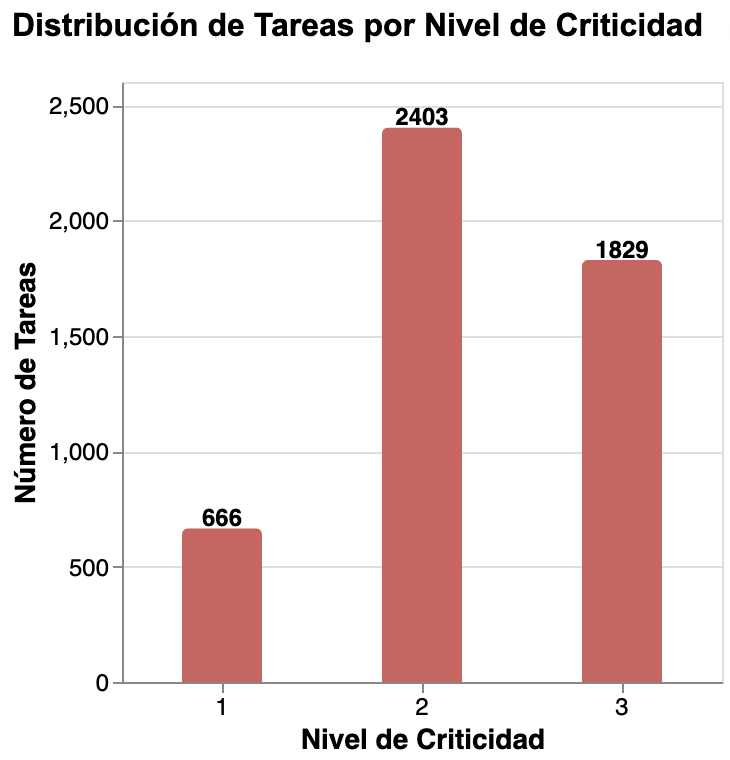
\includegraphics[width=0.5\textwidth]{imgs/barras_impacto.png}
    \caption{Distribución de tareas según su nivel de criticidad.}
    \label{fig:barras_impacto}
\end{figure}

Este dataset proporciona una base detallada y realista para el análisis y la implementación del modelo de programación, ya que combina un gran volumen de tareas con restricciones complejas y una diversidad de recursos. Además, la alta proporción de tareas con criticidad 1 y 2 subraya la importancia de optimizar el uso de los recursos para garantizar la ejecución de las tareas más críticas dentro de sus ventanas de tiempo establecidas

\subsection{Ajuste de Parámetros para la Función Objetivo}

La función objetivo del modelo combina dos componentes clave: el makespan, representado por el parámetro \( \alpha \), y la penalización por tareas no programadas, representada por el parámetro \( \beta \). Para determinar los valores más adecuados de \( \alpha \) y \( \beta \), se llevaron a cabo múltiples experimentos utilizando diferentes combinaciones de estos parámetros. El objetivo fue evaluar cómo cada configuración afecta el equilibrio entre la minimización del makespan y la cantidad de tareas programadas, especialmente aquellas con criticidad alta (impacto 1).

En estos experimentos, los resultados fueron analizados en función de métricas clave, incluyendo el número total de tareas programadas, la cantidad de tareas no programadas, el makespan obtenido, el tiempo de solución requerido y la cantidad de tareas no programadas según su nivel de impacto. Los resultados se presentan en dos tablas: la Tabla~\ref{tab:alpha_beta_general} resume las métricas generales, mientras que la Tabla~\ref{tab:alpha_beta_impact} detalla la distribución de tareas no programadas según su impacto.

\begin{table}[H]
    \centering
    \begin{tabular}{c>{\centering\arraybackslash}p{0.8cm} >{\centering\arraybackslash}p{0.8cm} 
                    >{\centering\arraybackslash}p{2.5cm} >{\centering\arraybackslash}p{2.5cm}
                    >{\centering\arraybackslash}p{2.5cm} >{\centering\arraybackslash}p{2.5cm}}
        \toprule
        \textbf{Conf.} & \( \alpha \) & \( \beta \) & 
        \makecell{\textbf{Tareas} \\ \textbf{Programadas}} & 
        \makecell{\textbf{Tareas no} \\ \textbf{Programadas}} & 
        \makecell{\textbf{Tiempo de} \\ \textbf{Solución (s)}} & 
        \textbf{Makespan} \\
        \midrule
        (a) & 1 & 0 & 0 & 4.898 & 3,43 & 0 \\
        (b) & 0 & 1 & 4.854 & 44 & 4,35 & 1.072 \\
        (c) & 1 & 1 & 4.658 & 240 & 8,42 & 492,75 \\
        (d) & 1 & 2 & 4.831 & 67 & 9,95 & 516,25 \\
        \bottomrule
    \end{tabular}
    \caption{Resultados generales obtenidos con diferentes configuraciones de \( \alpha \) y \( \beta \).}
    \label{tab:alpha_beta_general}
\end{table}


\paragraph{Resultados por Configuración}  
La configuración \( a \), donde \( \alpha = 1 \) y \( \beta = 0 \), prioriza exclusivamente la minimización del makespan. Sin embargo, este enfoque no logra programar ninguna tarea, lo que resulta inaceptable, ya que no se cumple el objetivo principal del modelo. Por otro lado, la configuración \( b \) (\( \alpha = 0 \), \( \beta = 1 \)) busca maximizar la cantidad de tareas programadas, logrando 4854 tareas en total. Aunque esta configuración presenta un makespan elevado (1072 unidades de tiempo), consigue programar todas las tareas de impacto 1, lo cual es un resultado favorable para las tareas más críticas.

La configuración \( c \) (\( \alpha = 1 \), \( \beta = 1 \)) equilibra ambos objetivos, pero a costa de una mayor cantidad de tareas no programadas (240). Si bien su makespan es menor que el de \( b \), su penalización por dejar tareas críticas fuera del cronograma lo hace menos atractivo.

Finalmente, la configuración \( d \) (\( \alpha = 1 \), \( \beta = 2 \)) logra un balance ideal entre los objetivos de programación y makespan. Con 4831 tareas programadas, esta configuración deja fuera solo 67 tareas, manteniendo el makespan en un nivel razonable de 516.25 unidades de tiempo. Además, se asegura que todas las tareas de impacto 1 son programadas, mientras que las tareas de impacto 2 y 3 no programadas son reducidas al mínimo posible.

\begin{table}[H]
    \centering
    \begin{tabular}{c>{\centering\arraybackslash}p{1.5cm} >{\centering\arraybackslash}p{1.5cm} 
                    >{\centering\arraybackslash}p{1.5cm}}
        \toprule
        \textbf{Conf.} & \makecell{\textbf{Impacto} \\ \textbf{1}} & 
        \makecell{\textbf{Impacto} \\ \textbf{2}} & 
        \makecell{\textbf{Impacto} \\ \textbf{3}} \\
        \midrule
        (a) & 666 & 2.403 & 1.829 \\
        (b) & 0 & 8 & 36 \\
        (c) & 21 & 59 & 160 \\
        (d) & 0 & 12 & 55 \\
        \bottomrule
    \end{tabular}
    \caption{Distribución de tareas no programadas según su impacto.}
    \label{tab:alpha_beta_impact}
\end{table}


\paragraph{Justificación de la Configuración Elegida}  
Se seleccionó la configuración \( d \) debido a su capacidad para satisfacer las prioridades del modelo. Aunque el tiempo de solución es el más alto entre las configuraciones evaluadas (9,95 segundos), este es un compromiso aceptable dado que garantiza un equilibrio óptimo entre la minimización del makespan y la programación de tareas críticas. Sin embargo, este tiempo de solución podría representar un desafío operativo en escenarios más grandes. Para abordar este problema, se propone utilizar la segmentación en subconjuntos, una técnica que divide el problema en partes más manejables, reduciendo así el tiempo de cálculo necesario para resolver cada subconjunto de tareas.

\paragraph{Visualización de los Resultados}  
Para ilustrar el efecto de los diferentes valores de \( \alpha \) y \( \beta \), se incluye la Figura~\ref{fig:alpha_beta_analysis}, que muestra el trade-off entre tareas programadas y el makespan en función de las configuraciones evaluadas. Este gráfico resalta cómo la configuración \( d \) logra un equilibrio favorable en comparación con las demás opciones.

\begin{figure}[H]
    \centering
    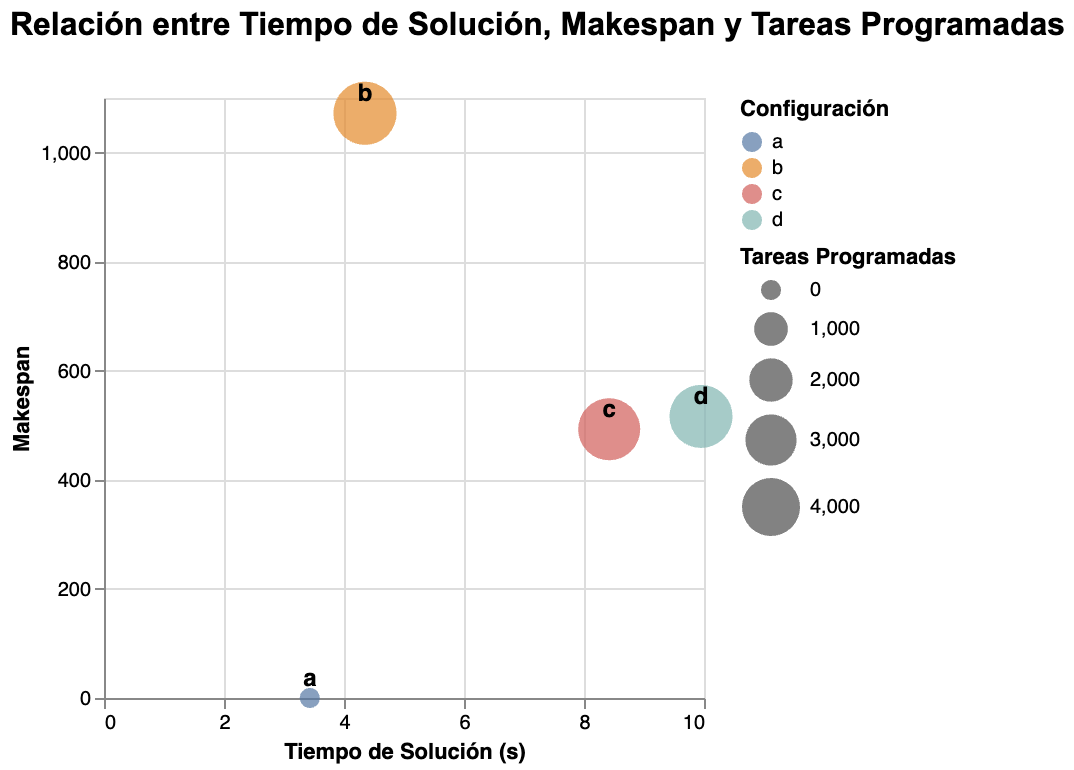
\includegraphics[width=0.7\textwidth]{imgs/sensibilidad_soluciones.png}
    \caption{Análisis de las configuraciones de \( \alpha \) y \( \beta \).}
    \label{fig:alpha_beta_analysis}
\end{figure}

En conclusión, la selección de \( \alpha = 1 \) y \( \beta = 2 \) se justifica por su desempeño superior en las métricas clave del modelo, alineándose con las prioridades operativas y estratégicas de la empresa. La implementación de la segmentación en subconjuntos permitirá optimizar aún más el tiempo de solución, asegurando que el modelo pueda escalar eficientemente a problemas más complejos.



\subsection{Resultados de la Segmentación en Subconjuntos}

La segmentación en subconjuntos permitió dividir el conjunto total de tareas en 14 subconjuntos más manejables, con el objetivo de reducir el tiempo de procesamiento del modelo. En la Tabla~\ref{tab:subsets_results} se presentan los resultados obtenidos, incluyendo el número de tareas en cada subconjunto, su porcentaje relativo con respecto al total (redondeado sin decimales) y el tiempo de solución requerido para resolver cada uno. Este análisis se llevó a cabo en un servidor virtual con las siguientes especificaciones:  

\begin{itemize}
    \item \textbf{vCPU/s:} 4 vCPUs.
    \item \textbf{RAM:} 8192 MB.
    \item \textbf{Almacenamiento:} 75 GB NVMe.
    \item \textbf{Sistema Operativo:} Ubuntu 24.10 x64.
\end{itemize}

\begin{table}[H]
    \centering
    \begin{tabular}{cccc}
        \toprule
        \textbf{Subconjunto} & \textbf{Número de Tareas} & \textbf{\% del Total} & \textbf{Tiempo de Solución (s)} \\
        \midrule
        \textit{S1} & 2.598 & 53\% & 4,34 \\
        \textit{S2} & 674 & 14\% & 0,65 \\
        \textit{S3} & 319 & 7\% & 0,43 \\
        \textit{S4} & 254 & 5\% & 0,12 \\
        \textit{S5} & 198 & 4\% & 0,01 \\
        \textit{S6} & 136 & 3\% & 0,01 \\
        \textit{S7} & 122 & 2\% & 0,00 \\
        \textit{S8} & 110 & 2\% & 0,01 \\
        \textit{S9} & 98 & 2\% & 0,00 \\
        \textit{S10} & 87 & 2\% & 0,00 \\
        \textit{S11} & 84 & 2\% & 0,01 \\
        \textit{S12} & 78 & 2\% & 0,00 \\
        \textit{S13} & 72 & 1\% & 0,00 \\
        \textit{S14} & 68 & 1\% & 0,00 \\
        \bottomrule
    \end{tabular}
    \caption{Resultados de la segmentación en subconjuntos.}
    \label{tab:subsets_results}
\end{table}


\paragraph{Distribución de Tareas}  
La segmentación produjo un subconjunto principal, \( S1 \), que contiene 2598 tareas, lo que equivale al 53\% del total. Este subconjunto representa más de la mitad de las tareas y, consecuentemente, requirió el mayor tiempo de solución (4.34 segundos). Por otro lado, los restantes 13 subconjuntos contienen entre 68 y 674 tareas cada uno, representando porcentajes significativamente menores del total.  

El segundo subconjunto más grande, \( S2 \), con 674 tareas (14\%), presentó un tiempo de solución de 0.65 segundos, lo cual destaca la eficiencia del enfoque modular al tratar con subconjuntos de menor tamaño. Los subconjuntos más pequeños, desde \( S5 \) hasta \( S14 \), contienen menos del 5\% de las tareas totales cada uno y se resolvieron en tiempos cercanos a cero segundos.  

\paragraph{Paralelización del Procesamiento}  
El procesamiento de los subconjuntos se realizó de manera paralela, aprovechando las capacidades del servidor utilizado. Como resultado, el tiempo total de solución fue igual al máximo tiempo de solución de todos los subconjuntos, es decir, 4.34 segundos. Este enfoque evidencia la ventaja de dividir el problema en partes independientes y resolverlas simultáneamente, reduciendo significativamente el tiempo total necesario para obtener los resultados.

\paragraph{Análisis de Desempeño}  
La segmentación permitió reducir notablemente los tiempos de solución al dividir el problema en partes más manejables. Aunque \( S1 \) sigue siendo considerablemente grande, su tiempo de solución es razonable gracias a la eficiencia del modelo implementado y a las especificaciones del servidor utilizado. Los subconjuntos más pequeños muestran un tiempo de solución despreciable, evidenciando que la segmentación fue efectiva en distribuir la carga computacional.  

\paragraph{Relevancia de la Segmentación}  
El análisis demuestra que más del 50\% de las tareas están concentradas en un único subconjunto (\( S1 \)), mientras que los demás subconjuntos están distribuidos de manera desigual, con tamaños que van disminuyendo gradualmente. Esto sugiere que ciertas tareas tienen conexiones más fuertes o restricciones compartidas, lo que explica la formación de un subconjunto dominante.  

Esta concentración implica que el tiempo de solución de \( S1 \) tiene un impacto considerable en el desempeño general del modelo. Sin embargo, el tiempo total de cálculo es altamente competitivo debido al enfoque de paralelización, que permite manejar incluso el subconjunto más grande sin afectar el tiempo general de procesamiento.

\paragraph{Conclusión sobre la Segmentación}  
La segmentación en subconjuntos demostró ser una estrategia efectiva para abordar el tiempo de solución del modelo, permitiendo resolver problemas complejos en tiempos razonables. El tiempo de solución total fue igual al máximo tiempo de solución de un subconjunto (4.34 segundos), gracias al procesamiento paralelo. En el futuro, podrían explorarse estrategias adicionales, como balancear aún más el tamaño de los subconjuntos o aplicar técnicas de optimización avanzada, para mejorar la eficiencia en escenarios con volúmenes de datos aún mayores.  


\subsection{Mejoras en la duración total del cronograma}

El análisis comparativo entre el cronograma generado manualmente y el producido por el solver muestra una reducción significativa en la duración total del proyecto (\textit{makespan}). Con los datos del conjunto original, el \textit{makespan} inicial era de 25,3 días, mientras que el modelo de optimización logró reducir este valor a 20,5 días, representando una mejora del 18,9\%. Este ahorro de tiempo no solo implica una mayor eficiencia en la ejecución de tareas, sino que también reduce el tiempo en que los equipos e instalaciones permanecen fuera de operación, impactando positivamente en los costos operativos.

\begin{table}[H]
\centering
\begin{tabular}{|c|c|}
\hline
\textbf{Indicador}            & \textbf{Valor}       \\ \hline
Makespan original             & 25,3 días           \\ \hline
Makespan optimizado           & 20,5 días           \\ \hline
Reducción en makespan         & 18,9\%              \\ \hline
\end{tabular}
\caption{Reducción del \textit{makespan} tras la optimización.}
\label{tab:makespan}
\end{table}

\subsection{Ahorros estimados en tiempo del equipo de programación}

Actualmente, el equipo de programación está compuesto por tres personas que dedican un promedio de 8 horas a la semana a la generación manual del cronograma. Con la implementación de esta herramienta, se estima que dicho tiempo podría reducirse considerablemente, ya que el solver automatiza gran parte del proceso, incluyendo la asignación de tareas y el balanceo de recursos. Esto representa un ahorro semanal estimado de 8 horas, que puede ser redirigido hacia otras actividades de mayor valor agregado, como la validación final o la coordinación con otras áreas.

Además, gracias a la capacidad del solver para realizar ajustes rápidos, el equipo podrá integrar tareas nuevas o modificar el cronograma de manera ágil, especialmente en situaciones donde surjan cambios inesperados en la planificación o disponibilidad de recursos. Esta funcionalidad es crucial para mantener la flexibilidad operativa y asegurar que el cronograma refleje las necesidades actuales en tiempo real.

\subsection{Impacto en la reducción de errores humanos}

Uno de los beneficios más significativos, aunque difícil de cuantificar en este momento, es la reducción de errores humanos. En los procesos manuales, es común que ocurran problemas como:
\begin{itemize}
    \item Recursos doblemente agendados.
    \item Cuadrillas asignadas a tareas sin los recursos necesarios.
    \item Equipos programados en horarios donde no están disponibles.
\end{itemize}

Estos errores pueden generar retrasos en las operaciones de mantenimiento, aumentando el tiempo de inactividad de los equipos. En un entorno productivo, estos tiempos adicionales pueden traducirse en costos significativos debido a la falta de disponibilidad de equipos críticos. La automatización del proceso con un solver minimiza estas situaciones, ya que se asegura de cumplir todas las restricciones operativas de manera estricta.

\subsection{Proyección de ahorros generales}

Aunque no se puede calcular un valor exacto, la reducción en errores y el aumento en la eficiencia del proceso tienen el potencial de generar ahorros importantes para la empresa. Al minimizar los problemas operativos y los tiempos de inactividad no planificados, se reduce el impacto financiero asociado al mantenimiento no eficiente. Además, la capacidad de actualizar rápidamente el cronograma reduce la dependencia de procesos iterativos y manuales, haciendo que el equipo de programación sea más productivo y eficiente.

\subsection{Pasos a seguir}

La solución se desarrolla de manera modular, estructurándose en tres componentes principales: el backend, el frontend y la integración con las plataformas de la empresa. Esta división permite organizar el flujo de trabajo de forma eficiente y facilita la colaboración con el equipo técnico de la empresa, asegurando que la solución se adapte adecuadamente a sus necesidades.

\begin{figure}[htbp]
  \centering
  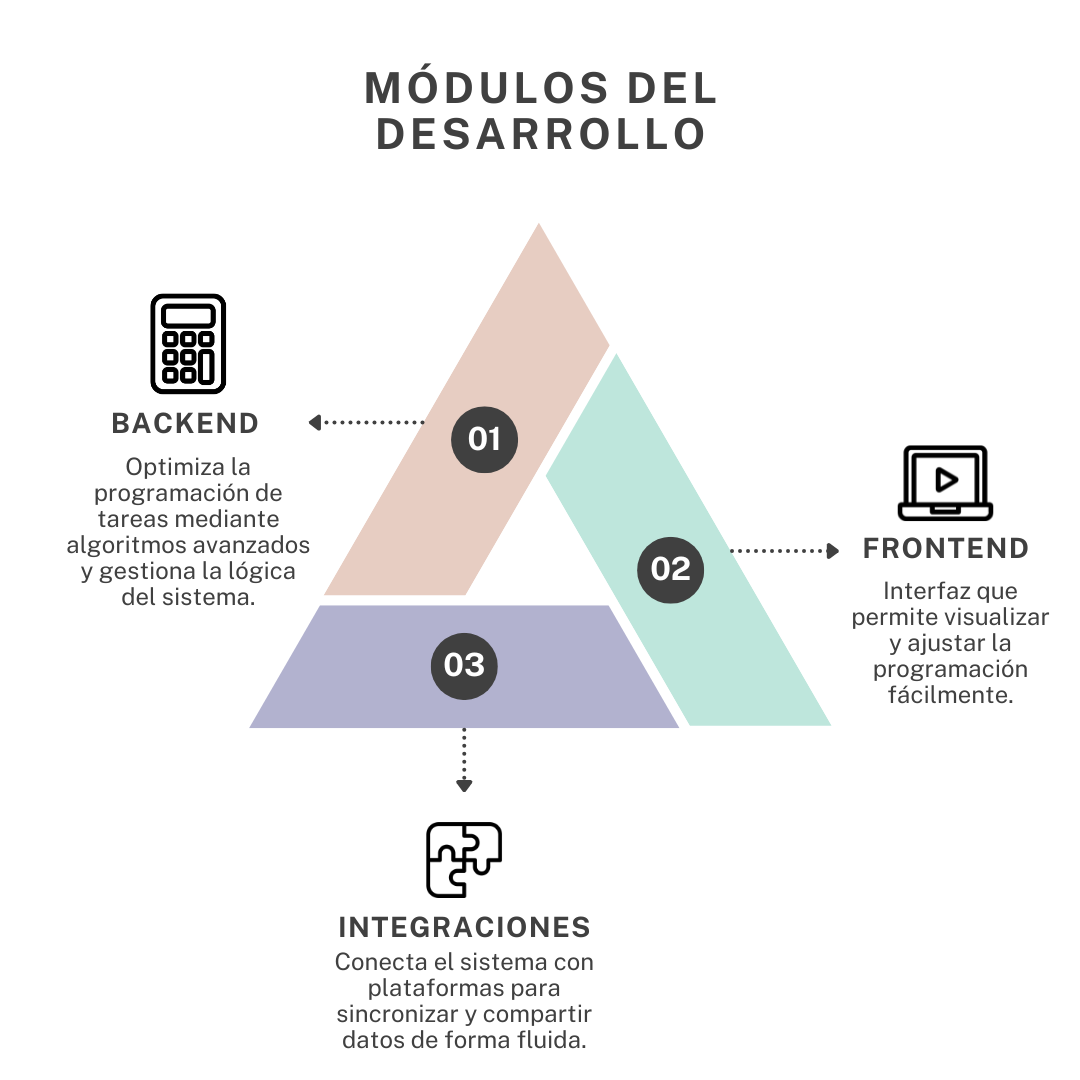
\includegraphics[scale=0.3]{imgs/ModulosDesarrollo.png}
  \caption{Módulos de Desarrollo de Solución}
  \label{fig:modulos-desarrollo}
\end{figure}


\subsubsection{Backend}

El backend representa el núcleo funcional de la solución y ejecuta el algoritmo de programación automatizada de tareas. Este algoritmo se selecciona en función de su capacidad para generar resultados de alta calidad que cumplan con las restricciones y optimicen la programación de tareas según los objetivos planteados. El backend recibe como entrada los datos de las órdenes de trabajo, que incluyen la información específica de cada tarea, tales como duraciones, recursos necesarios, precedencias y ventanas de tiempo.

Alojado en un servicio cloud de la empresa, el backend aprovecha la escalabilidad y el acceso seguro que este entorno proporciona. A partir de los datos ingresados, el backend genera como salida una programación detallada de tareas, especificando para cada una si fue programada y, en caso afirmativo, su hora de inicio. Este módulo se encarga de gestionar la lógica y optimización del proceso de programación, aplicando los algoritmos seleccionados, como CP-SAT, algoritmos genéticos u otros métodos heurísticos y metaheurísticos evaluados.

\subsubsection{Frontend}

El frontend funciona como la interfaz principal para los programadores de la empresa, quienes son los usuarios de esta solución. Su diseño se orienta a la facilidad de uso, permitiendo que los programadores carguen los datos de las órdenes de trabajo de manera sencilla. La carga de datos se puede realizar manualmente o mediante una integración con el sistema ERP de la empresa, de modo que los datos se incorporan automáticamente al sistema.

Una de las funciones clave del frontend es la visualización de la programación de tareas mediante una carta Gantt interactiva, que permite a los usuarios visualizar y, si es necesario, ajustar manualmente la programación generada. Esta funcionalidad ofrece a los programadores la capacidad de evaluar y modificar las tareas programadas antes de aprobar la versión final de la programación. Una vez aprobada, esta información se envía a la plataforma de la empresa, notificando a todos los involucrados sobre la programación establecida.

\subsubsection{Integración con Plataformas de la Empresa}

El tercer módulo se encarga de la integración de la solución con las plataformas de la empresa. Este componente se desarrolla en colaboración estrecha con el equipo de TI de la empresa, asegurando que los formatos de entrada y salida de los datos sean compatibles con los sistemas existentes. La integración también abarca la configuración de conexiones seguras entre el backend y las plataformas corporativas, permitiendo un flujo de información bidireccional. De esta forma, los datos de las órdenes de trabajo y de la programación finalizada se comparten con el ERP y otros sistemas relevantes de la empresa, facilitando la comunicación y coordinación entre los distintos equipos.



\subsection{Resumen de beneficios}

En resumen, los principales beneficios obtenidos mediante la implementación del solver son los siguientes:
\begin{itemize}
    \item Reducción del \textit{makespan} en un 18,9\%, optimizando la duración total del cronograma.
    \item Ahorro estimado de 8 horas semanales en tiempo del equipo de programación.
    \item Mayor flexibilidad para realizar ajustes rápidos y manejar cambios intempestivos en el cronograma.
    \item Reducción en errores humanos, mejorando la precisión de la programación y minimizando los costos asociados a problemas operativos.
\end{itemize}

Estos resultados preliminares destacan el potencial del modelo para transformar el proceso de programación, haciéndolo más eficiente, preciso y adaptado a las necesidades dinámicas de la operación.



\newpage

\begin{appendix}
    \section{Resultados Encuesta sobre Programación de Actividades en el Área de Mantenimiento de Anglo American Chile}
    \section*{Resumen Ejecutivo}

    Se realizó una encuesta a programadores del área de mantenimiento de las operaciones Los Bronces y El Soldado de Anglo American Chile, con el objetivo de identificar los principales desafíos y oportunidades de mejora en el proceso de programación. La encuesta abordó aspectos como dedicación horaria, actividades realizadas, errores comunes y problemas asociados a la coordinación.
    
    Las principales conclusiones son:
    
    \begin{itemize}
        \item \textbf{Alta dedicación horaria}: 64\% de los encuestados invierte más de la mitad de su jornada semanal en generación del cronograma de actividades.
        \item \textbf{La creación del borrador inicial} es la fase más intensiva en tiempo, superando otras actividades como resolver conflictos o validar con otras áreas.
        \item \textbf{La no disponibilidad de materiales y repuestos} durante la ejecución de las mantenciones es el error más recurrente.
        \item \textbf{Entorno altamente dinámico}: El 90\% de los encuestados enfrenta cambios de último minuto al menos una vez por semana.
        \item \textbf{Problemas de coordinación con otras áreas} y \textbf{falta de colaboración} son barreras adicionales que dificultan la programación eficiente.
    \end{itemize}
    
    Los resultados de la encuesta muestran que el proceso de programación podría beneficiarse significativamente de herramientas que automaticen partes claves del proceso. Una herramienta de automatización que permita generar el borrador inicial del cronograma, incorporar facilmente cambios de último minuto y realizar ajustes derivados de conflictos de recursos o validaciones \textbf{podría reducir en un 50\% la dedicación horaria del equipo de programación} en lo que respecta a la creación del cronograma de tareas. 
    
    Su éxito dependerá de su integración con las fuentes de información adecuadas, especialmente con bodega, para garantizar la disponibilidad de materiales y repuestos. Con información precisa y confiable, esta herramienta también \textbf{podría disminuir hasta en un 75\% los errores en las labores de mantenimiento derivados de una programación deficiente}.
    
    \section*{Metodología}
    
    La encuesta se aplicó a un total de 19 programadores de las operaciones Los Bronces y El Soldado de Anglo American Chile, mediante una plataforma on-line, durante el mes de Diciembre de 2024. Se trató de un cuestionario breve, compuesto por 7 preguntas. La mediana del tiempo de respuesta fue de aproximadamente 5 minutos y 30 segundos. 
    
    Las preguntas estuvieron diseñadas para estimar el tiempo dedicado a la programación, la distribución de dicho tiempo entre distintas actividades, la frecuencia e impacto de errores, y las condiciones cambiantes que inciden en la planificación.
    
    A continuación se presentan los resultados y el análisis de las respuestas obtenidas.
    
    \section*{Resultados de la Encuesta}
    
    En esta sección se presentan las preguntas realizadas a los encuestados junto con una tabla que resume los resultados obtenidos. Posteriormente, se incluye un comentario que analiza los datos presentados y destaca las principales conclusiones relacionadas con cada pregunta.
    
    \vspace{.5em}
    \subsubsection*{Pregunta 1: ¿Cuántas horas a la semana dedica el equipo de programación a generar el cronograma de tareas?}
    
    
    
    \begin{table}[H]
        \centering
        \begin{tabular}{lcc}
            \toprule
            \textbf{Rango de horas} & \textbf{Porcentaje} & \textbf{Cantidad} \\
            \midrule
            Menos de 10 horas & 5\% & 1 \\
            Entre 10 y 20 horas & 32\% & 6 \\
            Entre 20 y 40 horas & 53\% & 10 \\
            Más de 40 horas & 11\% & 2 \\
            \bottomrule
        \end{tabular}
        \label{tab:horas_semanales}
    \end{table}
    
    \paragraph{Comentario} Es notable que más de la mitad de los encuestados (53\%) dedica entre 20 y 40 horas semanales a la programación. Esto sugiere que la generación del cronograma de tareas consume una parte significativa de la jornada: en 64\% de los casos, más de la mitad de la semana laboral.
    
    
    \vspace{1.5em}
    \subsubsection*{Pregunta 2: ¿Qué porcentaje del tiempo total de programación está dedicado a las siguientes actividades?}
    \vspace{.5em}
    
    \begin{table}[H]
        \centering
        \begin{tabular}{lccc c}
            \toprule
            \textbf{Actividad} & \textbf{Promedio (\%)} & \textbf{Mínimo (\%)} & \textbf{Máximo (\%)} \\
            \midrule
            Generar el borrador inicial & 34.8 & 0 & 66\\
            Resolver conflictos de recursos & 23.8 & 10 & 70\\
            Validar con otras áreas & 19.7 & 10 & 40\\
            Realizar ajustes finales & 21.7 & 0 & 50\\
            \bottomrule
        \end{tabular}
        \label{tab:distribucion_actividades}
    \end{table}
    
    \paragraph{Comentario} Alrededor del 35\% del tiempo total de programación se concentra en la generación del borrador inicial, convirtiéndose en la actividad más demandante. Le siguen la resolución de conflictos de recursos y la realización de ajustes finales, con promedios cercanos al 24\% y 22\%, respectivamente. Cabe destacar que algunas personas reportan dedicar un 0\% de su tiempo a generar el borrador inicial o a realizar ajustes finales, lo que sugiere que estas etapas pueden ser asumidas por otras áreas o que ciertos roles se centran exclusivamente en validaciones o resolución de conflictos.
    
    \vspace{1.5em}
    \subsubsection*{Pregunta 3: ¿Cuántas personas del equipo participan activamente en la programación y qué porcentaje de su jornada diaria dedican a esta actividad?}
    
    A partir del análisis de las 19 respuestas obtenidas, se observa una gran variabilidad en el porcentaje de jornada diaria dedicado a la programación y en el número de personas involucradas. Las estadísticas resumen se presentan en la siguiente tabla:
    
    \begin{table}[H]
        \centering
        \begin{tabular}{lcc}
            \toprule
            & \textbf{Promedio} & \textbf{Desviación Estándar} \\
            \midrule
            Número de personas & 2.8 & 1.5 \\
            Porcentaje de jornada diaria (\%) & 64.2 & 30.3 \\
            \bottomrule
        \end{tabular}
        \label{tab:estadisticas_resumen_jornada}
    \end{table}
    
    \paragraph{Comentario} Estos resultados reflejan una dispersión significativa: en algunos casos, un equipo reducido (2 personas) dedica el 100\% de su jornada a la programación, mientras que en otros equipos, más numerosos, el porcentaje de tiempo invertido es mucho menor.
    
    
    \vspace{1.5em}
    \subsubsection*{Pregunta 4: ¿Con qué frecuencia ocurren cambios de último minuto en las tareas o recursos disponibles?}
    
    \begin{table}[H]
        \centering
        \begin{tabular}{lcc}
            \toprule
            \textbf{Frecuencia} & \textbf{Porcentaje} & \textbf{Cantidad} \\
            \midrule
            Varias veces por semana & 42\% & 8 \\
            Semanalmente & 47\% & 9 \\
            Pocas veces al mes & 5\% & 1 \\
            Rara vez & 5\% & 1 \\
            \bottomrule
        \end{tabular}
        \label{tab:cambios_ultimo_minuto}
    \end{table}
    
    \paragraph{Comentario} Casi un 90\% del equipo enfrenta cambios de último minuto al menos una vez por semana. Esto evidencia un entorno altamente dinámico y la dificultad de anteponerse a los imprevistos en el proceso de programación.
    
    
    \vspace{1.5em}
    \subsubsection*{Pregunta 5: Cuál de estos errores es el más comun durante el proceso de programación?}
    
    \begin{table}[H]
        \centering
        \begin{tabular}{p{7cm}cc}
            \toprule
            \textbf{Tipo de error} & \textbf{Porcentaje} & \textbf{Cantidad} \\
            \midrule
            Cuadrilla no disponible & 0\% & 0 \\
            Herramientas o Equipos no disponibles & 16\% & 3 \\
            Naves o Talleres no disponibles & 0\% & 0 \\
            Materiales o Repuestos no disponibles & 74\% & 14 \\
            Omisión de tareas críticas & 0\% & 0 \\
            El equipo sobre el cual se programó la mantención se encuentra ocupado & 11\% & 2 \\
            \bottomrule
        \end{tabular}
        \label{tab:errores_comunes}
    \end{table}
    
    \paragraph{Comentario} Lejos, el problema más recurrente identificado por los encuestados es la falta de materiales o repuestos disponibles, con un 74\% de respuestas. En segundo lugar, se encuentra la falta de herramientas o equipos disponibles; y en tercer la coordinación deficiente que genera conflictos al programar mantenciones en equipos ocupados.
    
    Por otro lado, es destacable que algunos factores potencialmente problemáticos, como la falta de cuadrillas o de talleres disponibles, no representan un obstáculo en este contexto, ya que ninguno de los encuestados los señaló como fuente de errores. De manera similar, la omisión de tareas críticas tampoco parece ser un problema recurrente, lo que sugiere que estos asuntos se encuentran relativamente resueltas en el proceso actual.
    
    \vspace{1.5em}
    \subsubsection*{Pregunta 6: ¿Qué otros errores considera que podrían ocurrir durante el proceso de programación?}
    
    Las respuestas a esta pregunta abierta señalaron como errores adicionales frecuentes la falta de coordinación con otras áreas, la inclusión de actividades de último minuto, y las dificultades para coordinar a los diferentes especialistas involucrados en una tarea. También se mencionaron problemas relacionados con la falta de repuestos y la indisponibilidad de equipos auxiliares, fechas de mantenciones variables, y cambios operacionales o provenientes de otras áreas. Además, se destacó la información deficiente desde bodega en relación con los repuestos.
    
    \paragraph{Comentario} En conjunto, estas respuestas cualitativas confirman nuevamente la existencia de problemas significativos relacionados con la disponibilidad de materiales y repuestos, en gran parte vinculados a la información deficiente proporcionada por bodega. Sin embargo, también se destacan con frecuencia los problemas de coordinación con otras áreas, que reflejan desafíos relacionados con la alineación de procesos y la colaboración entre equipos.
    
    \vspace{1.5em}
    \subsubsection*{Pregunta 7: En promedio, ¿cuántos de estos errores ocurren por mes?}
    
    \begin{table}[H]
        \centering
        \begin{tabular}{p{7cm}cccc}
            \toprule
            \textbf{Tipo de error} & \textbf{Promedio} & \textbf{Mínimo} & \textbf{Máximo} \\
            \midrule
            Cuadrilla no disponible & 3.5 & 0 & 10 \\
            Herramientas o equipos no disponibles & 3.9 & 1 & 12 \\
            Naves o talleres no disponibles & 2.7 & 0 & 10 \\
            Omisión de tareas críticas & 2.4 & 0 & 6 \\
            El equipo sobre el cual se programó la mantención se encuentra ocupado & 3.9 & 1 & 12 \\
            Materiales o repuestos no disponibles & 6.3 & 1 & 14 \\
            \bottomrule
        \end{tabular}
        \label{tab:errores_especificos}
    \end{table}
    
    \paragraph{Comentario}La falta de materiales o repuestos disponibles vuelve a ser un factor crítico, con un promedio superior a 6 eventos por mes. Esto confirma la relevancia de contar con información fidedigna e integrada sobre la disponibilidad de recursos para mejorar la eficiencia del proceso de programación. Le siguen en frecuencia la falta de herramientas o equipos disponibles y la ocupación de los equipos programados para mantenciones, con un promedio de 3.9 eventos por mes cada uno.
    
    \section*{Análisis y Conclusiones}
    
    El análisis de los resultados de la encuesta resalta varios aspectos críticos que afectan el proceso de programación de las actividades de mantenimiento de Anglo American Chile. Entre los hallazgos principales, destaca la alta dedicación horaria, con un 64\% de los encuestados invirtiendo más de la mitad de su jornada semanal en la generación del cronograma de tareas. La creación del borrador inicial se identifica como la etapa más demandante, representando en promedio el 35\% del tiempo total dedicado.
    
    El entorno de programación se caracteriza por ser altamente dinámico, con el 90\% de los encuestados reportando cambios de último minuto al menos semanalmente. Los errores más recurrentes están relacionados con la disponibilidad de materiales y repuestos, mencionados por el 74\% de los participantes, seguidos por la falta de herramientas y equipos auxiliares. Adicionalmente, los problemas de coordinación con otras áreas y la falta de colaboración surgen como barreras relevantes que dificultan la planificación efectiva.
    
    Los resultados de la encuesta muestran que el proceso de programación de actividades de mantenimiento \uline{podría beneficiarse significativamente de herramientas que automatizan partes clave del proceso}. En particular, una herramienta que automatice la creación del borrador inicial del cronograma y que permita incorporar de forma fluida cambios de último minuto o ajustes derivados de la resolución de conflictos de recursos y validaciones con otras áreas sería altamente efectiva. Una herramienta de este tipo, que facilite la incorporación rápida de modificaciones, \textbf{podría reducir hasta en un 50\% la dedicación horaria} de los equipos de programación a esta tarea, optimizando el uso de su tiempo.
    
    El éxito de esta herramienta, sin embargo, dependerá en gran medida de su integración con las fuentes de información de otras áreas de la empresa. En particular, será esencial conectarla con el área de planificación para acceder a información crítica sobre las tareas, como sus requerimientos de recursos, ventanas de tiempo (fechas de inicio más tempranas y fechas requeridas), y restricciones operativas. Además, será crucial integrarla con la información de bodega para garantizar la disponibilidad de materiales y repuestos, así como también con los datos sobre la disponibilidad de equipos. Es posible que se necesite revisar y ajustar los procedimientos de estas áreas para garantizar que la información sea precisa y confiable. Si se logra implementar una herramienta que integre estas funcionalidades y asegure la calidad de los datos, los \textbf{errores en las labores de mantenimiento derivados de una programación deficiente podrían reducirse en alrededor de un 75\%}.
    
    
\end{appendix}

\end{document}
